% ----------------------------------------------------------------
% Article Class (This is a LaTeX2e document)  ********************
% ----------------------------------------------------------------
\documentclass[10pt]{article}
\usepackage[british]{babel}  %% Language
\usepackage[a4paper, margin=1in]{geometry} %% margins
\usepackage{graphicx} % Graphics - allows import of images
\usepackage{float} % Allows for control of float positions
\usepackage[english]{babel}
\usepackage{algorithm}
\usepackage{algorithmic}
\usepackage[noend]{algpseudocode}

\usepackage{float}
\usepackage[bookmarks=true]{hyperref} % 
\usepackage{graphicx}
\usepackage[export]{adjustbox}
\usepackage{wrapfig}
\usepackage{datetime}
\newdate{date}{06}{04}{2022}

%----------------------------------------------------------------

% Title page

%----------------------------------------------------------------
\begin{document}
\title{A Secure and Privacy Preserving Telehealth Solution in Fog Environment }%
%%%%

\author{Srijeet \underline{Gopalan} \\ 20206283 \\ MSc in Cloud Computing}%
%% PLEASE UNDERLINE your surname as it appears in Moodle 

\date{\displaydate{date}}
\date{\today}%
% ----------------------------------------------------------------
\maketitle
% ----------------------------------------------------------------


%----------------------------------------------------------------
% abstract
%----------------------------------------------------------------

\begin{abstract} % 150 - 200 Words
 
The emergence of smart health facilitates readily available healthcare services. Increased demand for medical services, on the other hand, necessitates additional computing and storage resources near patients/users for smart sensing, analysis and processing. Fog computing (FC) is a rapidly evolving field that has come to the fore as a valuable addition to the cloud that can address issues such as unpredictable latency, resource constraints, confidentiality, and easy accessibility Since information can be easily stored and assessed relatively close to sources of information on native fog nodes, it is relatively safe as compared to cloud computing. Still, present fog models do have number of flaws, and they only focus on one of two things: accuracy of data obtained or low turnaround time, not both. This paper proposes SPATS, a Secure AES encryption enabled Privacy Assured Telehealth System that addresses privacy and security threats in a fog environment by integrating stacking classifier in fog devices and deploying it in a real world application of automatic health analysis. The AES encryption technology is used to ensure privacy and security from attackers while sensitive data is stored in cloud. A detailed experimentation and analysis has been done using EHR dataset from real-world medical services to assess the performance of SPATS. The results of the experiments reveal that the proposed system accurately predicts the health condition. When compared to existing machine learning techniques, the suggested approach achieves a better prediction accuracy.

\newline

\newline \textbf{ \textit{Key Terms--} Fog Computing, Privacy Preservation, Telehealth System, Stacking, Machine Learning, Real-time, AES Encryption}
\end{abstract}
% \begin{keyword}

% \end{keyword}

%----------------------------------------------------------------

% Table of contents

%----------------------------------------------------------------
\tableofcontents
\thispagestyle{empty}
\cleardoublepage
\setcounter{page}{1}

%----------------------------------------------------------------

% Main Headings Section

%----------------------------------------------------------------



\section{Introduction}  

According to medical reports, 133 million people in the United States currently suffer from chronic illnesses. More than 171 million people are expected to be added by 2030. \cite{1}. As a result the popularity of smart health has emerged, with the goal of promoting easily accessible medical services through the use of advanced network and intelligent machines in smart cities. These services make use of the Internet of Things to link up large numbers of devices as well as people all over the world. The amount of interconnected devices is rapidly expanding, and by 2021, it will have surpassed 12 billion \cite{0}.
Since IoT devices have limited memory and processing capacity, they must often send large and diverse data to remote servers or cloud servers for processing. 
\newline

Integration of cloud computing within smart healthcare allows for considerably better data analysis as well as processing, however cloud computing faces several potential obstacles. Pushing a huge volume of data to cloud for computation causes latency as well as network utilisation issues \cite{3}.  A critically ill person, for instance, may collapse and require rapid medical attention. The remote server may fail to receive and process vital information in a timely manner, resulting in serious healthcare service failure. Moreover limiting the transmission speed of an infectious disease requires coordinating local area network or local resources with a remote server. As a result, the use of cloud computing in Smart healthcare programs reduces overall system's efficiency. In order to engage in smart health efficiently, critical telehealth processes should be processed and stored near to its users.
\newline

Fog computing is a type of cloud computing that could handle and archive large amounts of data generated by IoT devices close to their source. Fog computing's primary concept is to bring cloud services closer to IoT devices. As seen in Figure \ref{fig:1}, it serves as a bridge between the cloud and IoT devices. The fog layer serves as an intermediary layer, performing few of the processing as well as storage prior to data being transferred to the cloud \cite{2}.Fog computing may be appropriate for facilitating critical telehealth systems because of these qualities. Towards this, a hybrid of cloud and fog computing can provide a long-term solution to problems in today's healthcare systems.
\newline

\begin{figure}[H]
    \begin{center}
        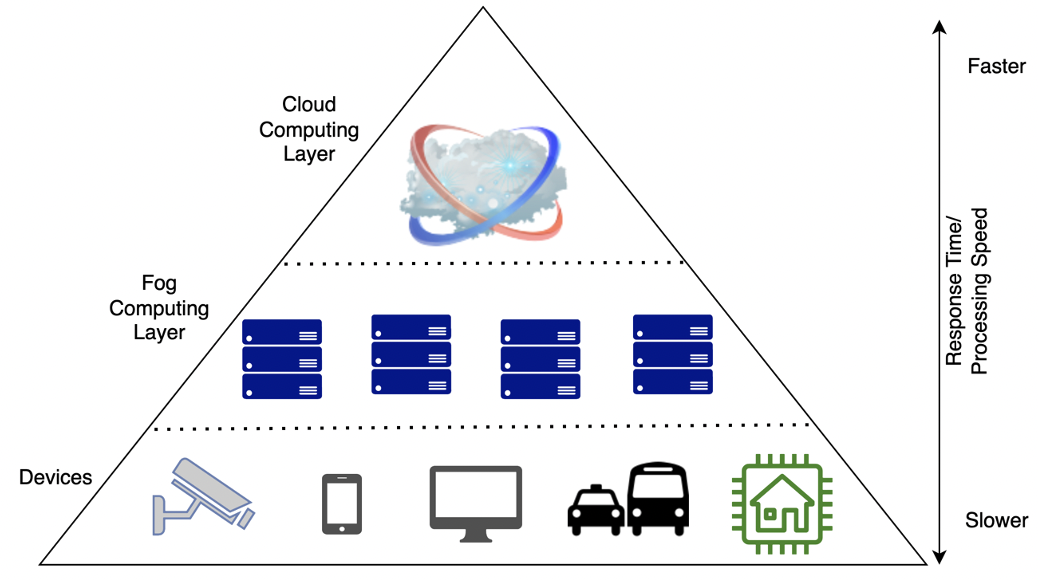
\includegraphics[width=0.7\linewidth,frame]{CA2-template/RIC1.png}
        \caption{Fog Computing Layers\label{fig:1}}
    \end{center}
\end{figure}


\subsection{Motivation}

Fog computing is one of the advanced technologies that helps to promote telehealth applications because these systems have become latency-sensitive but also faster in data processing, decision making and real-time tracking,  and are crucial factors in any healthcare system. The use of fog in healthcare has been the subject of numerous research. This inspires the development of a fog-based telehealth system. Health data is significant since it contains vital and confidential information. The goal of fog computing is to enable patients to manage their own health data on a local level.
\cite{4}. 

\subsection{Aim and Objectives}
\begin{itemize}
    \item To enhance the effectiveness and reliability of the telehealth systems by maintaining data close to the devices and applications,
\item To permit users to exchange data in real time environment and enabling safe storage of the data
\item To resolve the flaws of cloud-based health system
\end{itemize}


\subsection{Research Question}
\textbf{Can a fog-based telehealth system that embraces the AES encryption algorithm and the Stacking classifier optimize health assessment, maintain data security, anonymity, and provide real-time solutions?}
\newline

The rest of the paper is structured as follows: Section II, outlines the Literature Review, discusses the research aim and objectives, and highlights the intended contributions. The methodological approach is described in Section III, followed by design specification in Section IV and its implementation in Section V. Section VI presents the evaluation results and lastly Section IV draws the final conclusion.


\section{Literature Review} 

Several studies have been conducted to build a secure, fast and reliable tele-health system. However no previous contributions, specifically address the needs of integrated computing solutions in healthcare industry. 

\newline

Considering cloud as well as fog computing developments in the healthcare sector, there have been major contributions from various researchers. The literature review in this paper also looks at the limits of the associated studies. The taxonomy in Figure \ref{fig:2}, divides this section in three sub sections. 

\begin{figure}[H]
    \begin{center}
        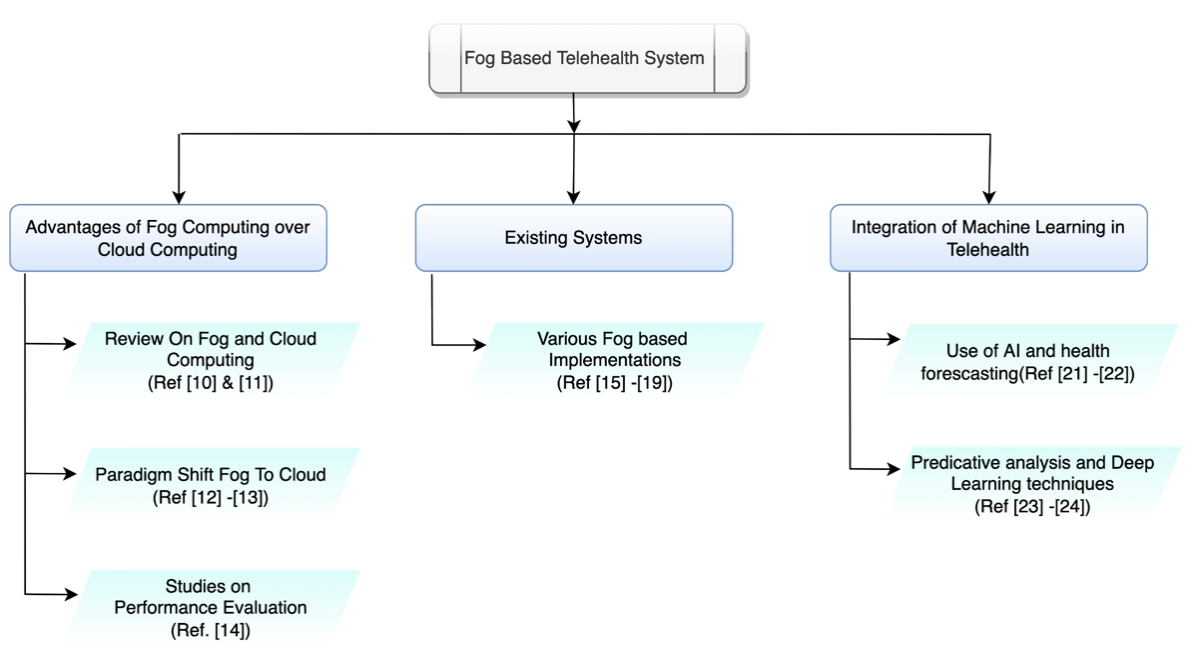
\includegraphics[width=1\linewidth,frame]{CA2-template/RIC2.png}
        \caption{Taxonomy\label{fig:2}}
    \end{center}
\end{figure}

\subsection{Advantages of Fog Computing over Cloud Computing}

A study revealed that a reasonably large majority of healthcare organisations prefer to employ cloud computing services to stay competitive by leveraging its advantages. Contrarily, cloud computing poses a number of challenges for the healthcare industry, including high bandwidth requirements, latency, operational issues, technological challenges, privacy challenges, and legal and regulatory concerns \cite{7}.
\newline


The ultimate approach for empowering the Internet of Things to deliver a secure and dependable service may well be fog computing. 
The whole fog computing model, along with levels, is covered in \cite{10}, along with an overview of various computing paradigms and traits. 
IoT and cloud computing integration, however, present a number of challenges. The framework of fog computing is also discussed by the researchers of \cite{11} as a potential solution to the issues of Cloud-IOT, including high latency as well as bandwidth, operating with numerous protocol suites, and others. 
\newline

The benefits, difficulties, and drawbacks of edge-cloud computing are covered in \cite{12}. 

Regarding security, design and architecture as well as protocol specifications, it presents ample opportunities for researchers. The report, however, does not account for the patterns as well as trends in cloud computing.In a nutshell, the report offered very little insight into the difficulties and possibilities presented by recent advances in cloud computing. On the other hand, \cite{13} helps to give future researches who are interested in the topic of handling the data in IOT, a place to start. Additionally, it covers the advantages and restrictions of fog computing as well as the utilisation of big data and IoT in a variety of applications. 

\newline
\newline


\subsection{Existing Systems}

The fog-based healthcare system was demonstrated for the detection of patients with Chikungunya virus (CHV) infection \cite{15}. 
The CHV virus can be monitored and detected by the system. A innovative system based on fog is described that uses FCM clustering to accurately classify people as either likely sick or unaffected by CHV and send diagnostic updates to the smartphone/device of the user.
The outcomes demonstrate the advantages of incorporating FC and CC services in order to obtain high throughput, outstanding QOS, and quick real-time warning issuance when compared to a cloud-only solution. The goal of the study was to produce an enhanced network throughput, good service, and the quickest response time for real-time alert \cite{15}. The proposed system's security and privacy aspects are not considered in the study. As a result, the article offered very little insight into the security difficulties. 
\newline

A home hospitalisation system was presented in \cite{17} that uses IOT alongwith fog and cloud computing to allow patients to get care and undergo rehabilitation from their homes, as their medical state and other parameters are monitored. 
The technology described in this study is noteworthy for its low cost, speed, and security and also for its capability to solve serious hospital problems. This system, however cannot transmit the data in real-time. So to assist the administration as well as telemonitoring of elderly patients on basis of health status, another fog based system is proposed in \cite{18}. 
Its performance is assessed using the FogWorkflowSim toolkit, proving that fog computing boosts the effectiveness of the entire system. However, it doesn't use any access control or security measures to maintain the system's anonymity.
\newline
\newline


\subsection{Integration of Machine Learning in Telehealth}

In order to predict possible health-related occurrences, the area of forecasting known as "health forecasting" has recently emerged \cite{22}. By encouraging medical practitioners to implement effective vulnerbility-reduction and supply management in advance, it supports precautionary medicine as well as healthcare intervention strategies. 
Making the best decisions for the health could help the user receive more appropriate care. In order to minimize hospital readmission rates, predictive analytics within healthcare can help determine critical patients at the home itself and save unnecessary down times \cite{23}. It can also help detect early signs of patient deterioration in the critical care unit. 
Predictive analytics should be adopted more quickly in the healthcare sector in order to improve nursing experience, chronic health condition treatment, and supply chain effectiveness.  
\newline 
\newline
\subsection{Research Niche}
The previous models and solutions, mentioned above, attempted to create a real-time, secure telehealth system, but they were unable to find a final solution that would have satisfied all of the goals, as was evident from the discussions above. Most of these required properties are achieved with fog computing. Therefore, a fog-based setting with a few small adjustments can achieve all of the design goals. The suggested architecture ensures secure data storage in the telehealth system using AES encryption techniques.
\newline
\newline

\section{Research Methodology} 
This section goes into great detail about how the SPATS gives its users the ability to recognize the severity of their health report and the type of treatment needed by using their own lab test results. The system's sequence diagram is shown in Figure \ref{fig:3}.

A thorough explanation of the four key stages of the system is as follows

\begin{figure}[H]
    \begin{center}
        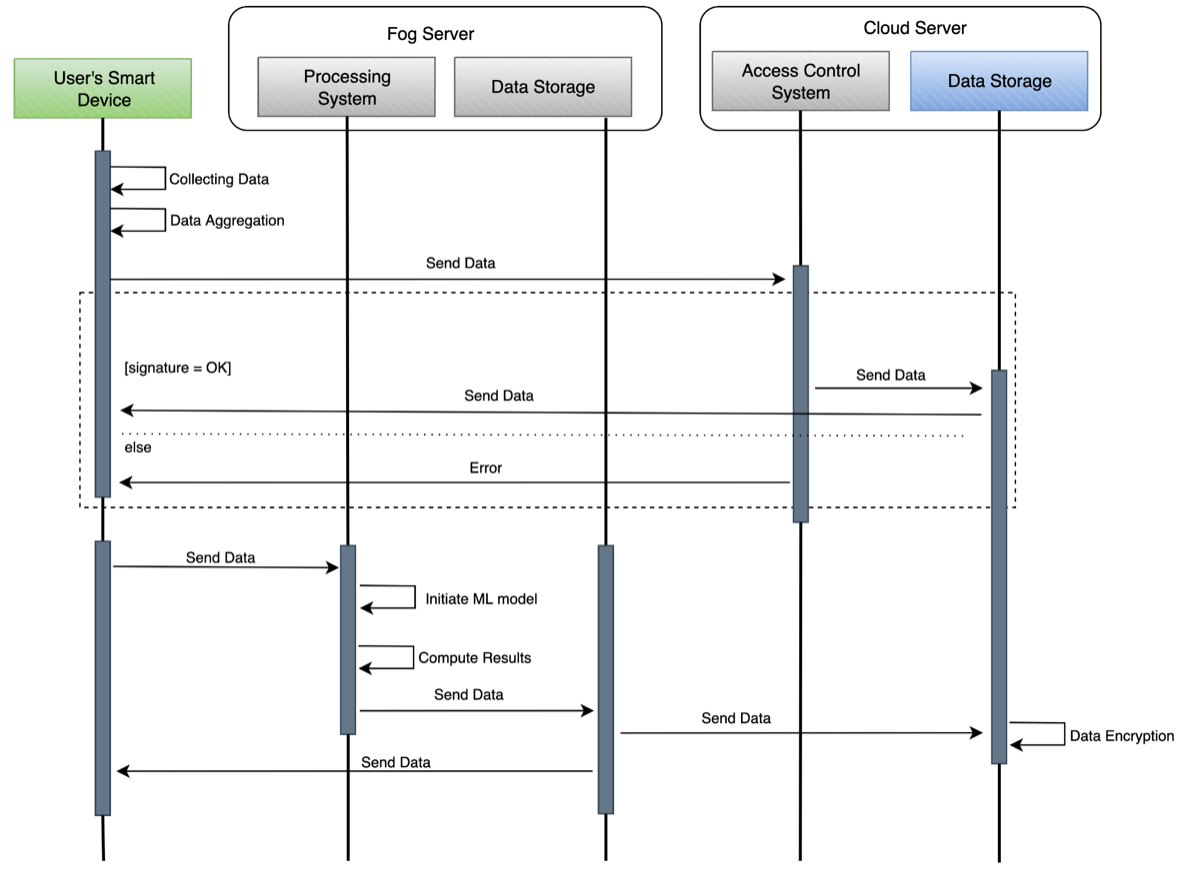
\includegraphics[width=0.9\linewidth,frame]{CA2-template/RIC3.png}
        \caption{Sequence Diagram\label{fig:3}}
    \end{center}
\end{figure}


\begin{description}
\item[User Registration/Authorization Stage]
To use the system's services, a new user may sign up to the SPATS web application to store the results on cloud or use the gateway application directly to check the results at a time. The registered user receives a user ID after completing the registration process via the web application, which is also needed to submit the lab test data and obtain the results. Once registered, the user can submit data or access past test results by entering his or her login information. However an unregistered user cannot view their past test results

\item[Data Capture Stage]
The users can enter the lab test report data and their credentials using the application installed on the fog device through their smart device. It sends the information on for processing. The post-processing findings are immediately sent back to the application. The system also compares the entered credentials to those in the database of registered users, and if a match is made, it sends the information to the cloud for long-term archiving. Even if the system is compromised, the encrypted format in which this data is kept in the cloud will prevent any data breaches.

\item[Data Processing Stage]
The ML algorithm processes the user's submitted data to assess the user's health condition and establish the standard of care required for the user.

\item[Final Stage]
The results are displayed to the user in real time at this stage, and they are also permanently saved in the cloud server. When needed, the user can log in to the SPATS web application and obtain their results. The AES encryption method is used to encrypt the data in the cloud to protect and preserve the privacy of the users.


\end{description}

\section{Design Specifications} 

The design specification of the fog based tele-health solutions in SPATS is described in this Section. The technological foundation of SPATS is explained first. Followed by a description of its architectural design model. Lastly the proposed machine learning algorithm is presented along with the application model in depth.

\subsection{Technological Foundation}
The resources utilised to implement SPATS are as follows:

\subsubsection{Coding Platform}
The SPATS cloud application is published using the integrated development environment (IDE) and dynamic staging ground of the Visual Studio 2019 Community edition. It offers an integrated development environment (IDE), a powerful programme with many features that may be utilised for various software development tasks. The development of SPATS has been made easier by Visual Studio's inclusion of compilers, autocomplete and graphical designing tools, and many other features in addition to the conventional editor as well as a debugger that are offered by the majority of IDEs. Additionally, Visual Studio makes it simple to publish applications to Azure's cloud \cite{25}.

\subsubsection{Cloud Service Provider}
SPATS leverages Microsoft's Azure cloud computing platform.  
It is built to operate on Microsoft's worldwide network and is It is used to create, manage, and deploy apps and services. Additionally, it is an open and customizable cloud platform that enables working on a worldwide network simpler by facilitating speedy creation, management, and deployment of applications. SPATS's cloud layer is based on Azure.

\subsubsection{Tool Used For Simulation}
For simulating a fog based system, there aren't many simulation tools available. Since iFogSim is the most prominent simulation tool in fog computing, this paper use it for performance evaluation of SPATS. The popular cloud computing simulator, CloudSim served as the foundation for the creation of iFogSim, which incorporates all of CloudSim's pertinent features and components. iFogSim, which can track several performance characteristics including energy usage, delay, speed of response, expense, etc., has a strong support system from research group. Additionally, it enables tests to be repeated in a regulated setting. 
\cite{26}.

\subsubsection{Encryption Algorithm Used}
Encryption is used to secure user data in the cloud. 
CSP alone is unable to give each user at every level a good encryption granularity. Therefore, a user-initiated encryption solution is required to secure personal data of SPATS users. AES symmetric cryptosystem is opted because it can quickly and effectively manage the encryption of enormous amounts of data. 
This encryption method doesn't require any changes in the application and can be rapidly and easily integrated. Thus, it guarantees that both data and encryption keys stay under the control of the user and are never revealed while being stored.

Figure \ref{fig:4} shows the process. It starts with clear-text, or unprotected data often called a message. The message is then converted from unencrypted to encrypted message, which is finally decrypted to return to human readable text.
\begin{figure}[H]
    \begin{center}
        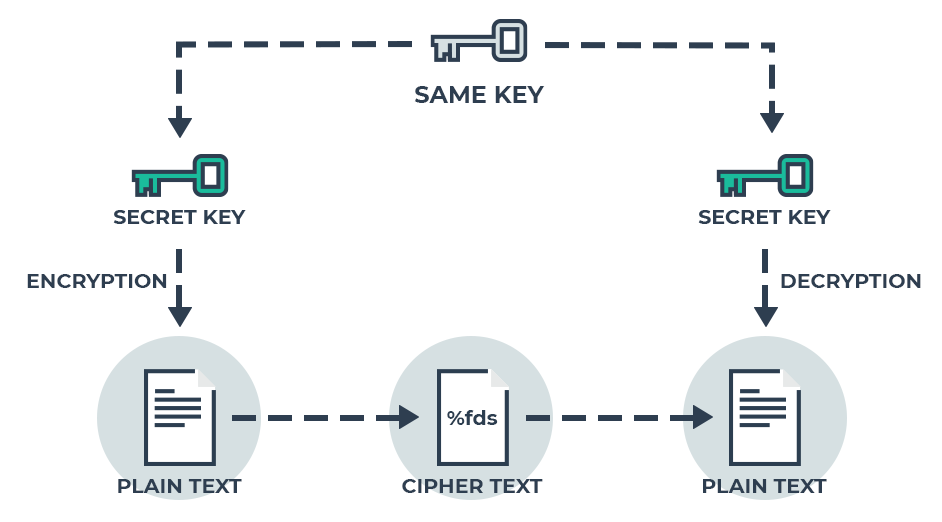
\includegraphics[width=0.7\linewidth,frame]{CA2-template/R3.png}
        \caption{The Process of Cryptography\label{fig:4}}
    \end{center}
\end{figure}

\newline

\subsection{SPATS System Model}
The SPATS system model consist of the the user module, the fog module and the cloud module. It is explained in detail in the following section Figure \ref{fig:4.1} shows a streamlined framework this model. 

\begin{figure}[H]
    \begin{center}
        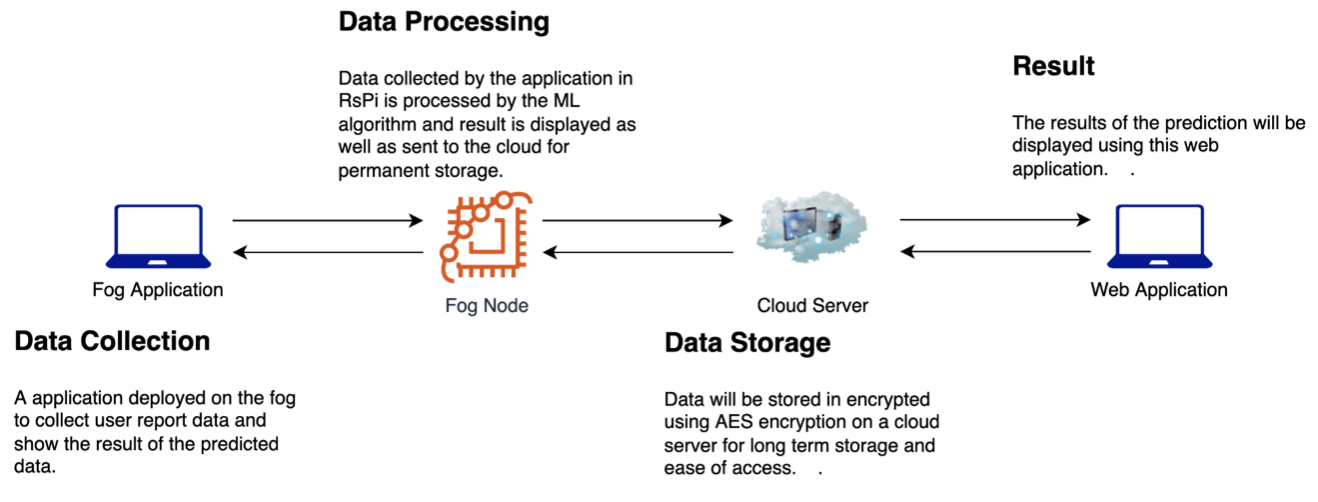
\includegraphics[width=0.9\linewidth,frame]{CA2-template/RIC18.png}
        \caption{Streamlined Framework\label{fig:4.1}}
    \end{center}
\end{figure}

\subsubsection{The User Module}
All registered users of this smart tele-health system have access to the User module of SPATS, which provides an interface via which they can communicate and exchange the necessary data. The user can access this telehealth system using a PC, a smartphone/tablet, or both. A sequence of questionnaires with fields for inputting report data are then displayed by the system and the communicated to the fog-server once the data is submitted. The information is initially provided by the user, and after that, it is forwarded to the fog server for additional processing. Additionally, users will be able to view their results also.

\subsubsection{The Fog Module}
The processing of user's data in real-time depends heavily on the Fog module. The user's device can send data to this fog module, which can then process it, store it, and produce results in accordance. Fog nodes are situated nearer to the users who wants to access the system, which speeds up data transmission and lowers latency caused by the network. 
As a fog node, SPATS employs Raspberry Pi 4 Model B with 4 GB RAM and 32GB SD card for storage.

Once it has been established whether the patient needs in-hospital critical care or at-home care, the information is sent back to the user's device for real-time display and is also sent to the medical-database in the cloud server. 


\paragraph{Data Summary}
Datasets are essential to machine learning. Among the most difficult tasks is data collecting, which is probably even more difficult when used in medical fields like early diagnosis.The SPATS uses a publicly available open dataset \cite{27}.
It is an EHR dataset obtained from one private health center in Indonesia. It includes the patient's lab results, which are used to establish the patient's condition and treatment plan, whether they are in-care or out-care patients. The data types used to express the numerous parameters to be verified in order to ascertain the user's health status are summarized in Table \ref{table:3}. The collection contains the laboratory test results for both healthy and critically ill users. 

\begin{table}[H]
\centering
\caption{Data types in EHR dataset\label{table:3}}
\begin{tabular}{|l|l|l|l|}
\hline
\textbf{S. No.} & \textit{\textbf{Attribute Name}} & \textbf{Attribute Type} & \textbf{Brief Description} \\ \hline
1 & HAEMATOCRIT & Float & Haematocrit level from a lab test results \\ \hline
2 & HAEMOGLOBINS & Float & Haemoglobins level from a lab test results \\ \hline
3 & ERYTHROCYTE & Float & Erythrocyte level from a lab test results \\ \hline
4 & LEUCOCYTE & Float & Leucocyte level from a lab test results \\ \hline
5 & THROMBOCYTE & Float & Thrombocyte level from a lab test results \\ \hline
6 & MCH & Float & MCH level from a lab test results \\ \hline
7 & MCHC & Float & MCHC level from a lab test results \\ \hline
8 & MCV & Float & MCV level from a lab test results \\ \hline
9 & AGE & Integer & Age of the patient \\ \hline
10 & SOURCE & Nominal & \begin{tabular}[c]{@{}l@{}}The category values are "in" for \\ hospital care patient and "out" for \\ home care patient.\end{tabular} \\ \hline
\end{tabular}

\end{table}

\paragraph{Model for Stacking Ensemble Learning}
The majority of the time, Base-learners construct ensemble learning employing a number of heterogeneous or homogeneous learners where prediction outputs are aggregated. The several sorts of combination methods are training, polling, and averages. Multiple base learners at first stage are connected to a meta-learner at the second stage by stacking.
To take full advantage of its heterogeneity, which is a key factor in creating a successful ensemble model, the three Base-learner used are: Random Forest (RF), XG Boost and meta-learner being ADA boost. Figure \ref{fig:5} provides a brief overview of the steps of this process
\begin{figure}[H]
    \begin{center}
        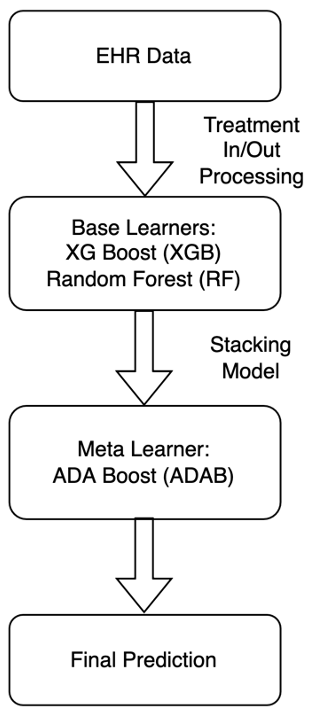
\includegraphics[width=0.18\linewidth,frame]{CA2-template/RIC4.png}
        \caption{The Process of Stacking Classifier\label{fig:5}}
    \end{center}
\end{figure}

\subsubsection{The Cloud Module}
This module uses Azure cloud storage and stores two different sorts of information. The user's Name, Email ID, Mobile Number, and Password are initially recorded in the registration data. Second, the results that were predicted by the fog module's model training. An automated User Id is generated for each user. With their ID, each user creates and stores a sizeable amount of data. The cloud module has high-end storage servers installed. 
\subsection{SPATS security features}
Although security requirements are an essential part of any cloud or fog architecture, there aren't many methods offered for creating secure applications. The confidentiality of user's personal medical data when it is preserved on cloud servers is provided by SPATS using following algorithms for encryption \ref{alg:enc} as well as decryption process \ref{alg:dec}. 

\begin{algorithm}[H]
\caption{AES Encryption Algorithm}\label{alg:enc}
\begin{algorithmic}
\Procedure{AddRoundKey}{$Message\ ,\ \&\ w\left[0\right]$}
\FOR{$i = Step\ 1\ to\ 9$}
\State $SubBytes(Message)$
\State $ShiftRows(Message)$
\State $MixColumns(Message)$
\State $AddRoundKey\left(Message\ ,\ \&w\left[i\ \times4\right]\right)$
\ENDFOR
\State $SubBytes(Message)$
\State $ShiftRows(Message)$
\State $AddRoundKey\left\left(Message\ ,\ \&w\left[40\right]\right)$
\end{algorithmic}
\end{algorithm}

\begin{algorithm}[H]
\caption{AES Decryption Algorithm}\label{alg:dec}
\begin{algorithmic}
\Procedure{AddRoundKey}{$Message\ ,\ \&\ w\left[0\right]$}
\FOR{$i = Step\ 1\ to\ 9$}
\State $InvSubBytes(Message)$
\State $InvShiftRows(Message)$
\State $InvMixColumns(Message)$
\State $AddRoundKey\left(Message\ ,\ \&w\left[i\ \times4\right]\right)$
\ENDFOR
\State $InvSubBytes(Message)$
\State $InvShiftRows(Message)$
\State $AddRoundKey\left\left(Message\ ,\ \&w\left[40\right]\right)$
\end{algorithmic}
\end{algorithm}

\section{Implementation}
Several programming languages were used to accomplish the elements described in Section 4. Python was used to implement the processing as well as machine learning parts. The gateway interface is built using Flask. The web application is built on ASP.NET framework using C# language and the database is on MySQL. Figure \ref{fig:4.1}  shows the actual setup of SPATS

\begin{figure}[H]
    \begin{center}
        \includegraphics[width=0.7\linewidth,frame]{CA2-template/RIC19.jpg}
        \caption{SPATS Deployed \label{fig:4.1}}
    \end{center}
\end{figure}



\subsection{Web Application}
This application, which is hosted on the Azure cloud and was developed using the ASP.NET framework and a SQL database, is accessible whenever the user wants to view the results of his or her predictions. Additionally, it is utilized to sign up to the SPATS system.The registered user will receive a UserID which can then be used on the gateway application to submit the report data and store the results on the cloud.

\subsubsection{Login and Registration Page}
The SPATS cloud application is accessible from this page, where the new users can register and current users can sign in. Validation rules are in place for SignUp. Invalid entries are not permitted as shown in Figure \ref{fig:6}
\begin{figure}[H]
    \begin{center}
        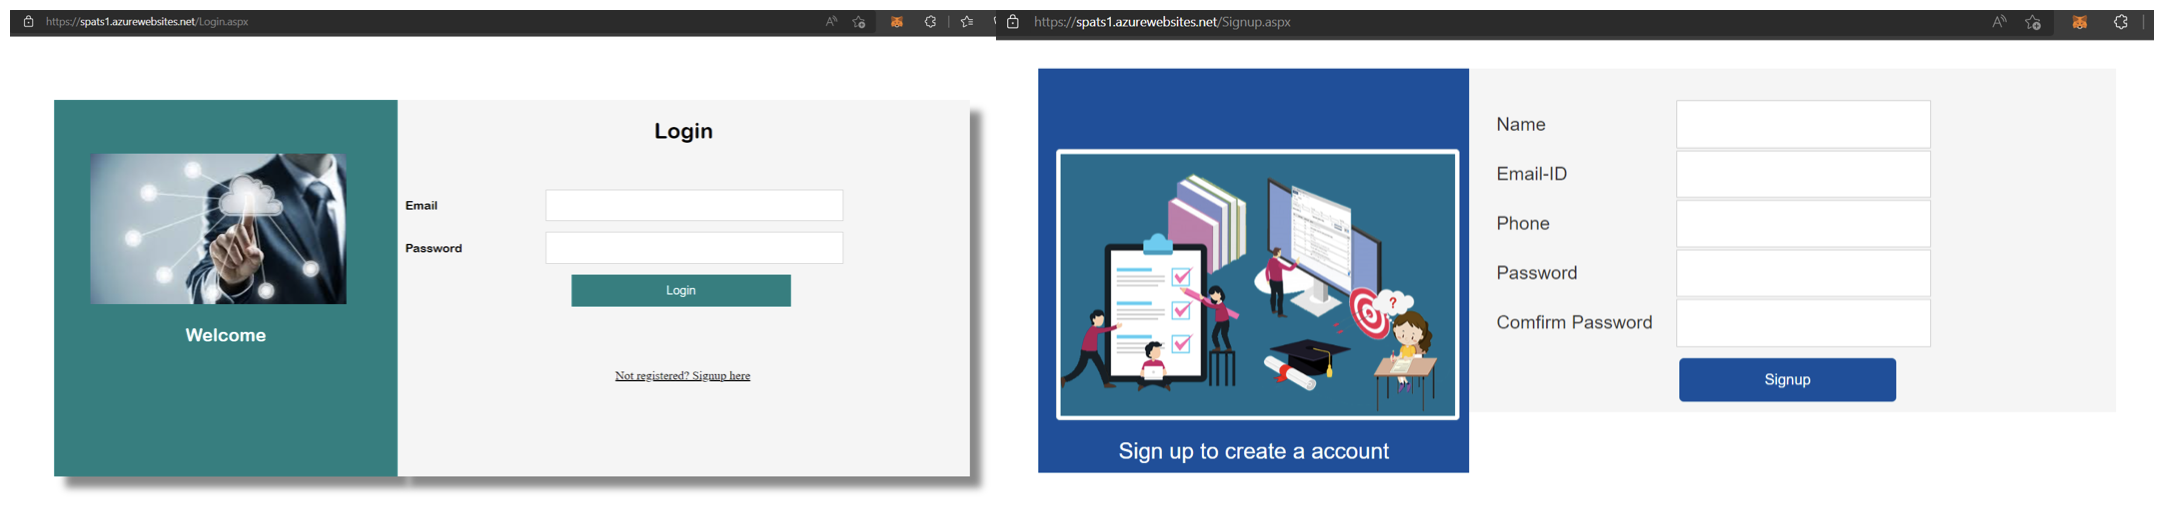
\includegraphics[width=0.9\linewidth,frame]{CA2-template/RIC5.png}
       
    \end{center}
\end{figure}
\begin{figure}[H]
    \begin{center}
        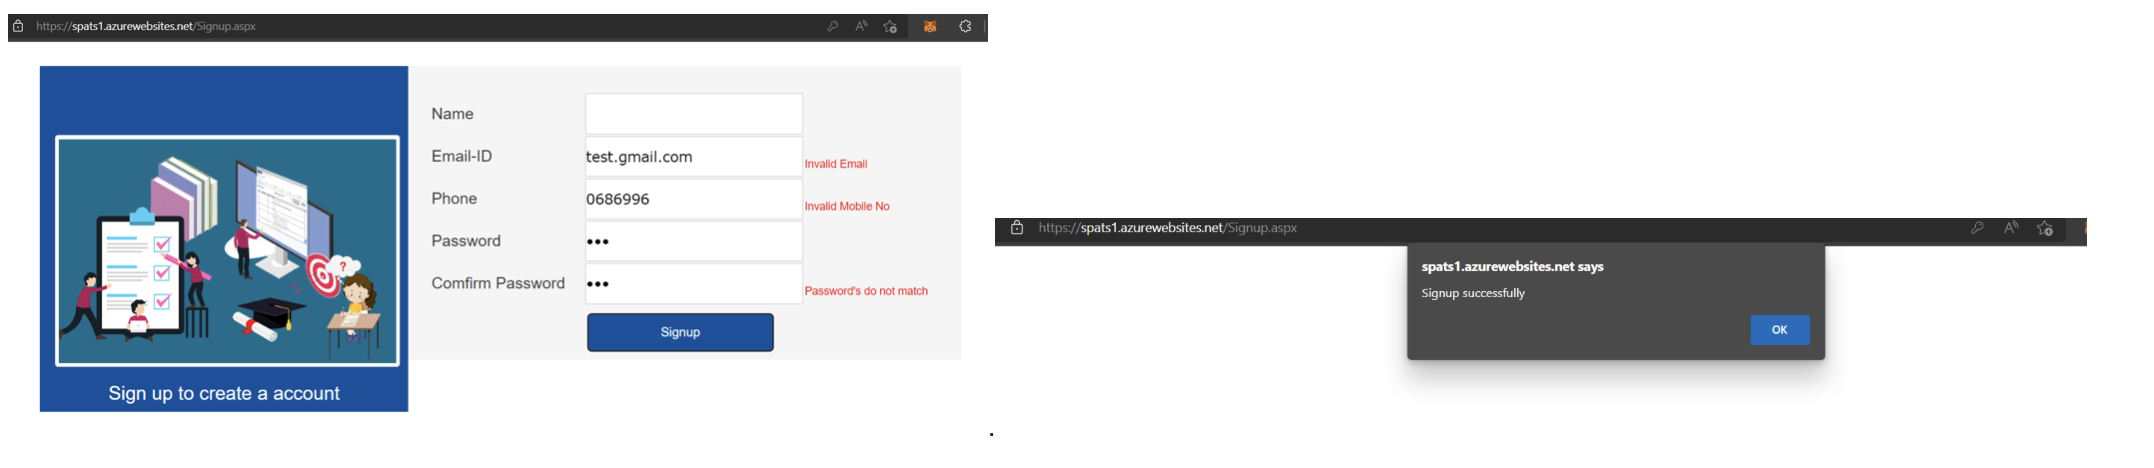
\includegraphics[width=0.9\linewidth,frame]{CA2-template/RIC6.png}
        \caption{Validation in Signup Page \label{fig:6}}
    \end{center}
\end{figure}

\subsubsection{Home and Result Page}
The UserID will be visible on the Home page once the user has successfully logged in. After selecting the Result tab from the left pane, a page with a list of submitted lab reports and their results will appear. By default, the results will be encrypted, to decrypt them, select the Decrypt button at the top. This displays the data in a format that is readable by humans as shown in Figure \ref{fig:7}
\begin{figure}[H]
    \begin{center}
        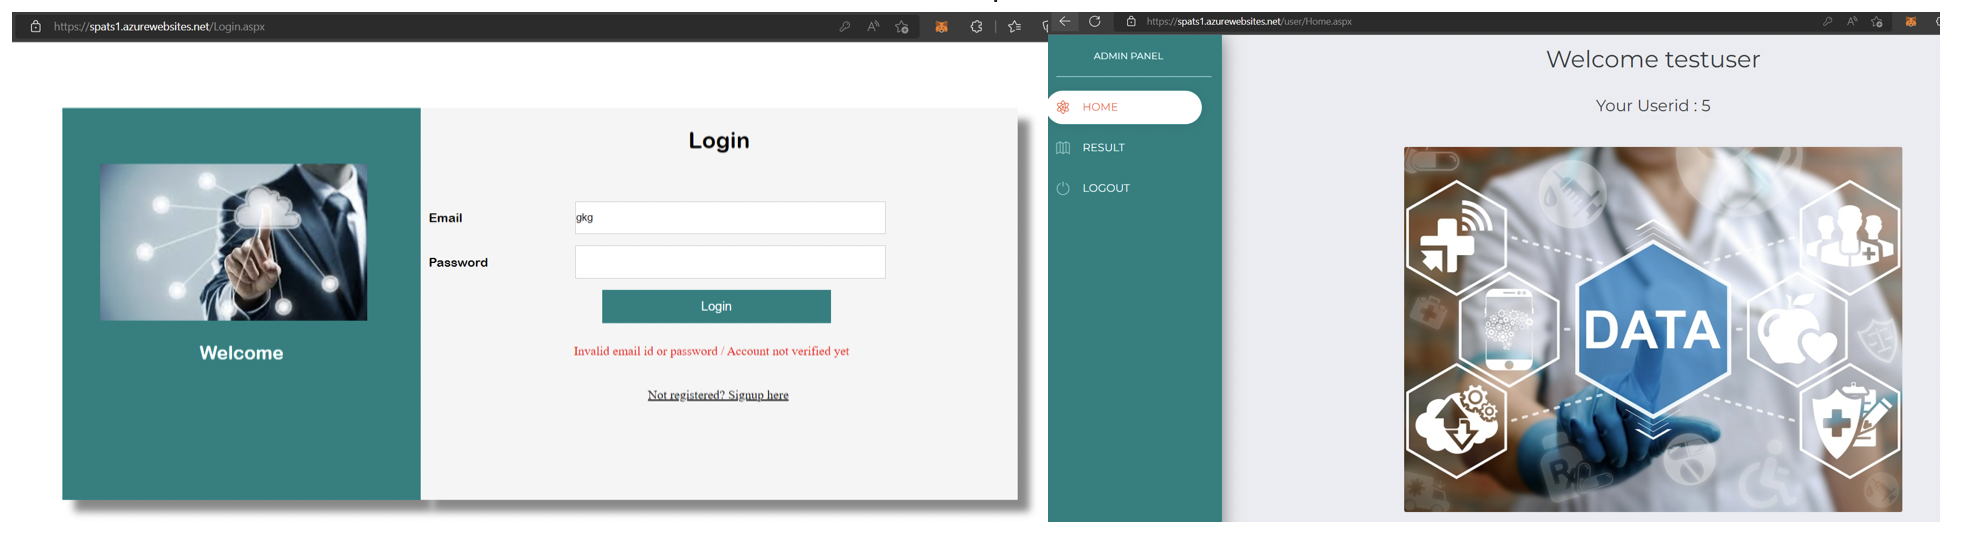
\includegraphics[width=0.9\linewidth,frame]{CA2-template/RIC7.png}
       
    \end{center}
\end{figure}
\begin{figure}[H]
    \begin{center}
        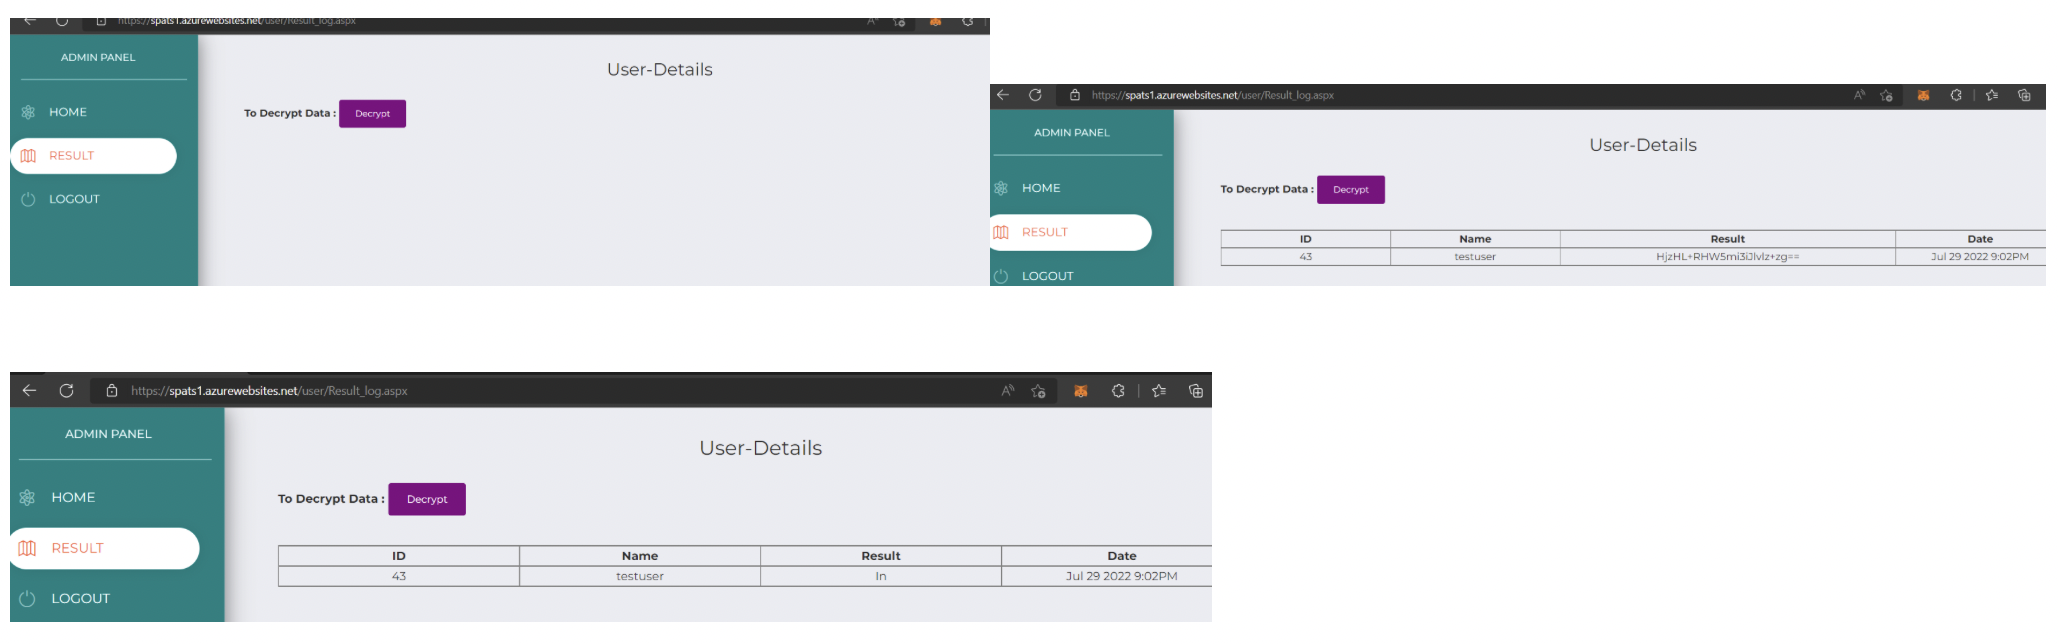
\includegraphics[width=0.9\linewidth,frame]{CA2-template/RIC8.png}
        \caption{Home and Result Page \label{fig:7}}
    \end{center}
\end{figure}

\subsection{Gateway Application}
The Flask Python framework was used to create this application, which is run on a Raspberry Pi. It includes machine learning models to assess the user's condition using models developed from the EHR dataset. The user can access this app on their smart devices and use it to submit the results of their lab tests in order to find out what kind of treatment is necessary for them based on the submitted report data.

\subsubsection{Homepage}
The homepage has a button named predict to redirect to the prediction page and, if scrolled down, a brief description of the SPATS is also provided as shown in Figure \ref{fig:8}
\begin{figure}[H]
    \begin{center}
        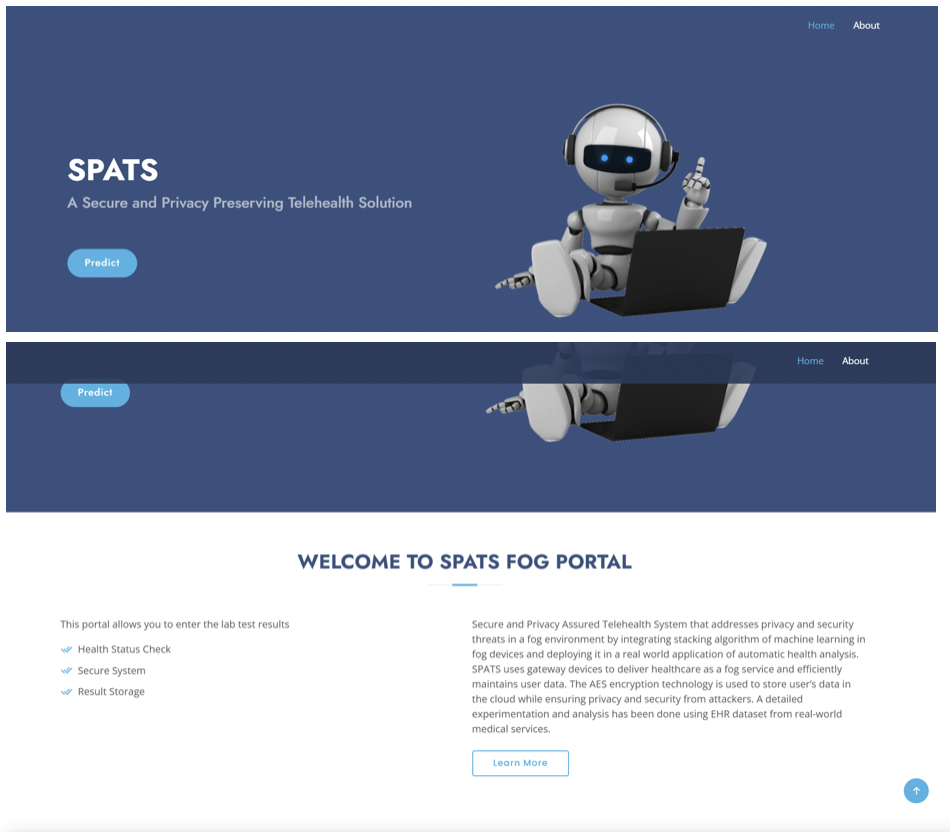
\includegraphics[width=0.9\linewidth,frame]{CA2-template/RIC9.png}
       \caption{Home page \label{fig:8}}
    \end{center}
\end{figure}

\subsubsection{Results}
This page shows a form with a list of fields for entering the data of the lab test as shown in Figure \ref{fig:9}
Both registered and unregistered users will be able to see the result, but only registered users' results will be saved to the cloud.

\begin{figure}[H]
    \begin{center}
        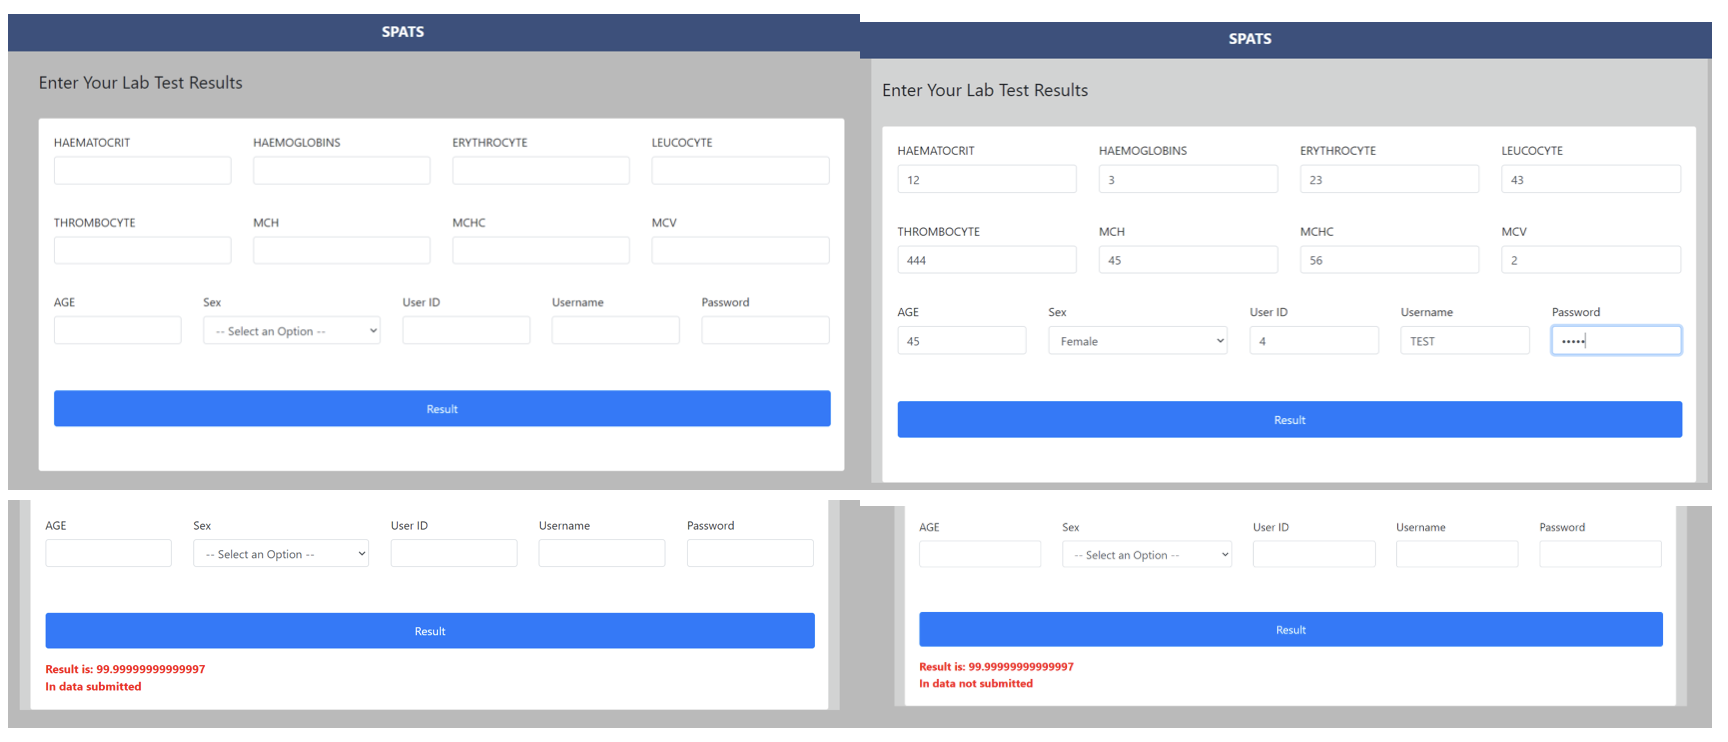
\includegraphics[width=0.9\linewidth,frame]{CA2-template/RIC10.png}
       \caption{Results \label{fig:9}}
    \end{center}
\end{figure}

\section{Evaluation}
The evaluations are conducted in two phases to test the efficiency of both the system and the classifier used for training the data models. In order to assess the latency and bandwidth consumption, the full framework is first simulated in IFogSim toolkit and the results are captured. In second phase, the classifier is assessed for precision, accuracy as well as there ROC graphs.

\subsection{Evaluating the Performance of SPATS}
As a testing ground for the SPATS framework's model evaluation, iFogSim Tookit is employed. The CloudSim-libraries will be included in order to run the simulation. There are two different situations for the simulation. In the first case, the cloud subsystem receives data from the IoT subsystem via the intermediary fog subsystem. To retrieve data, a request will be sent and thus data is fetched via the cloud component and fog component, respectively. And in second situation, the fog component is not involved and the data created is sent straight to the cloud component. 

In order to obtain a clear trend, three configurations shown in Table \ref{table:4}are used with varying numbers of smart devices and fog units. Each parameter's experimental findings are shown and described.

\begin{table}[H]
\centering
\begin{tabular}{|c|c|c|}
\hline
\multicolumn{1}{|l|}{\textbf{Configuration}} & \multicolumn{1}{l|}{\textbf{Units/Fog node(s)}} & \multicolumn{1}{l|}{\textbf{Smart Device(s)}} \\ \hline
C1 & 1 & 2 \\ \hline
C2 & 2 & 4 \\ \hline
C3 & 3 & 6 \\ \hline
\end{tabular}
\caption{Configuration Scenarios \label{table:4}}
\end{table}


\subsubsection{Bandwidth Consumption}
The suggested framework's bandwidth usage is shown in Figure \ref{fig:11}. As number of smart devices has increased, there is a subsequent increase in network demand when only a cloud component is used. However w hen the fog component was included, network consumption decreased slightly.
\begin{figure}[H]
    \begin{center}
        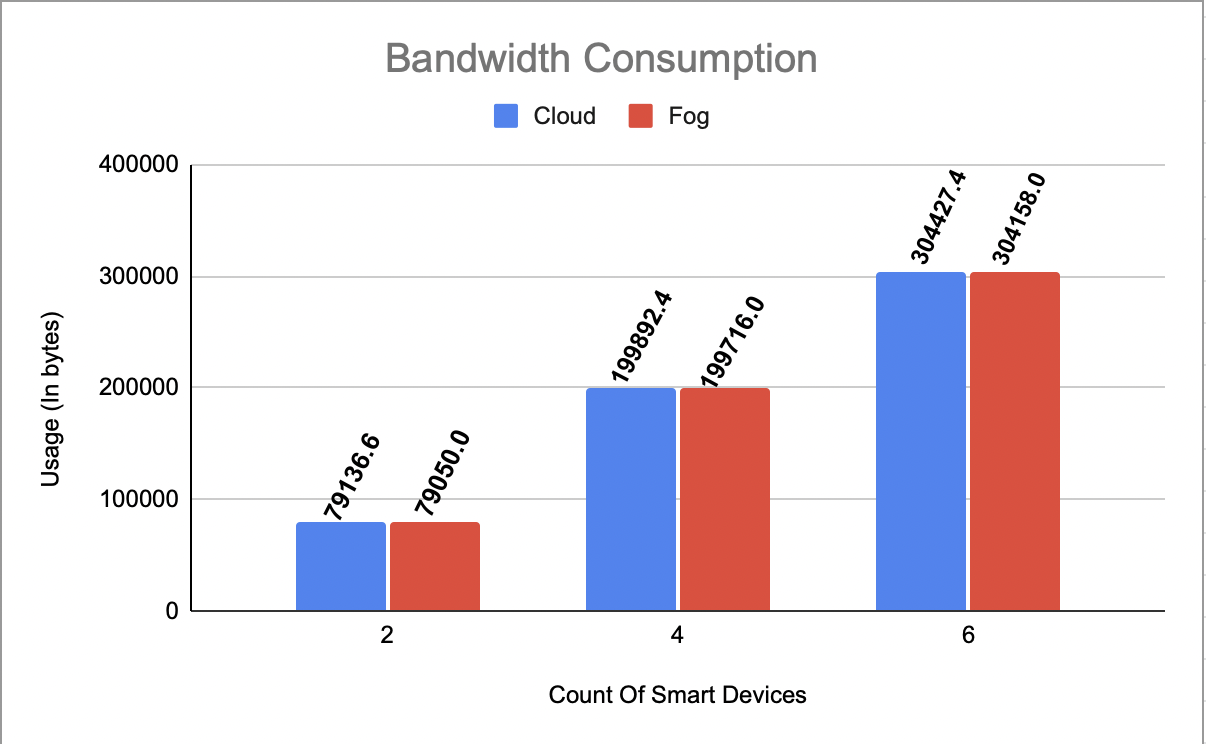
\includegraphics[width=0.7\linewidth,frame]{CA2-template/RIC11.png}
       \caption{Bandwidth Consumption \label{fig:11}}
    \end{center}
\end{figure}


\subsubsection{Latency}
The latency is measured as the total turnaround time for transmitting data from the smart device to the fog unit and back. These time measurements are depicted graphically in Figure \ref{fig:10} for both the instances, first with a fog component present and the second, without one.
\begin{figure}[H]
    \begin{center}
        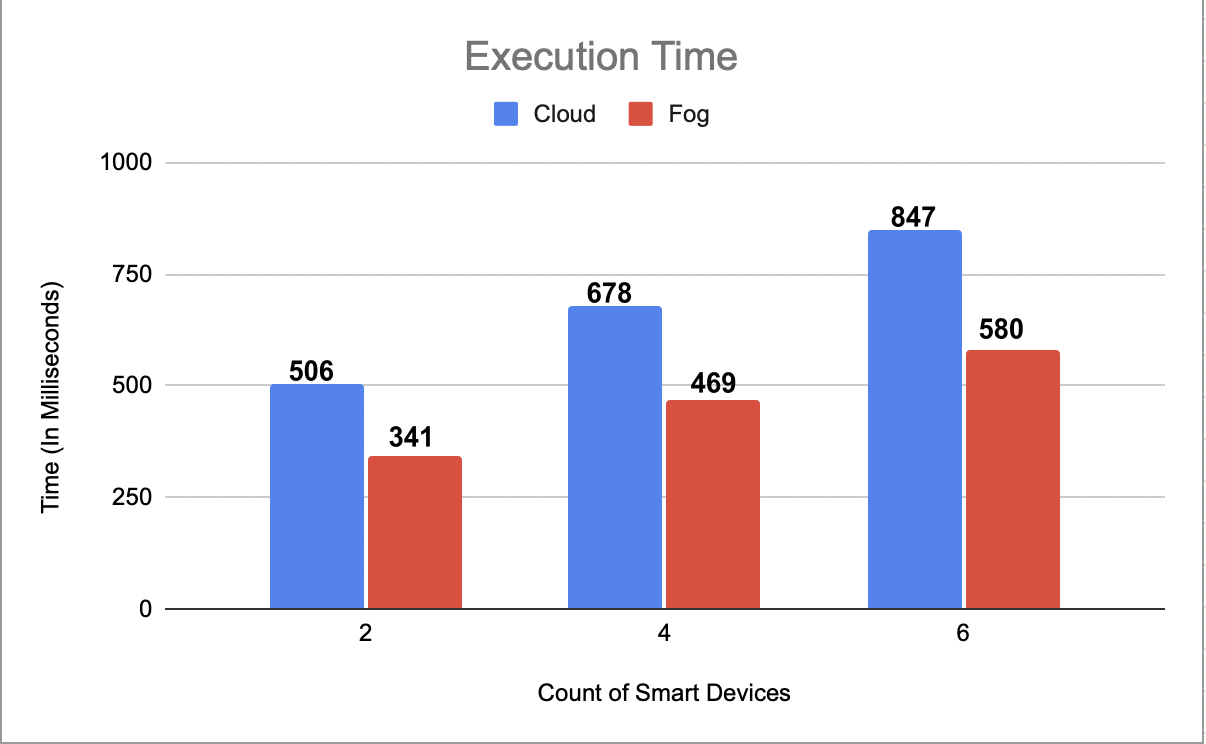
\includegraphics[width=0.7\linewidth,frame]{CA2-template/RIC12.png}
       \caption{Latency \label{fig:10}}
    \end{center}
\end{figure}

\subsection{Stacking classifier's performance evaluation}
A classification model's performance evaluation is an important stage since it demonstrates how effective is classifier. 
70 percent of the dataset is used for training, while twenty percent is used for testing. Machine learning-related libraries and Python language are used for data operations. Pandas is being used for data processing, quick accessibility of data, and simple data operations. The model training as well as the evaluation stages involve the use of Scikit-learn, an open-source toolkit that offers complete AI techniques. Matplotlib, NumPy, and SciPy, three complete libraries enabling numerical computation with Python, are the foundations upon which Pandas or rather Scikit-learn are based.

\subsubsection{Precision}
Precision measures how often true positive values occur among all positive values. Figure \ref{fig:14} demonstrates that the stacking classifier outperforms existing traditional classifiers.
\begin{figure}[H]
    \begin{center}
        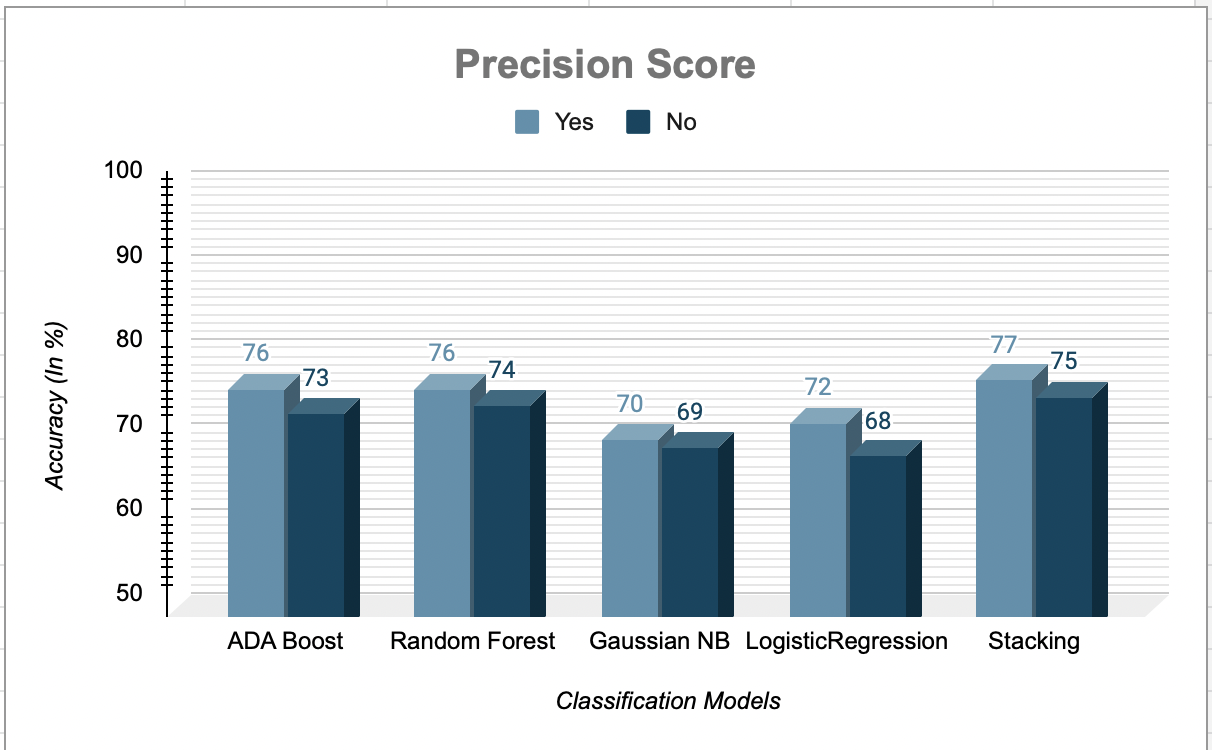
\includegraphics[width=0.7\linewidth,frame]{CA2-template/RIC14.png}
       \caption{Precision \label{fig:14}}
    \end{center}
\end{figure}


\subsubsection{Accuracy}
The primary factor to consider when evaluating a classifier is its accuracy. By assessing the percent of true predictions, it demonstrates effectiveness. Figure \ref{fig:13} clearly demonstrates that the stacking classifier outperforms conventional classifiers in terms of outcomes.

\begin{figure}[H]
    \begin{center}
        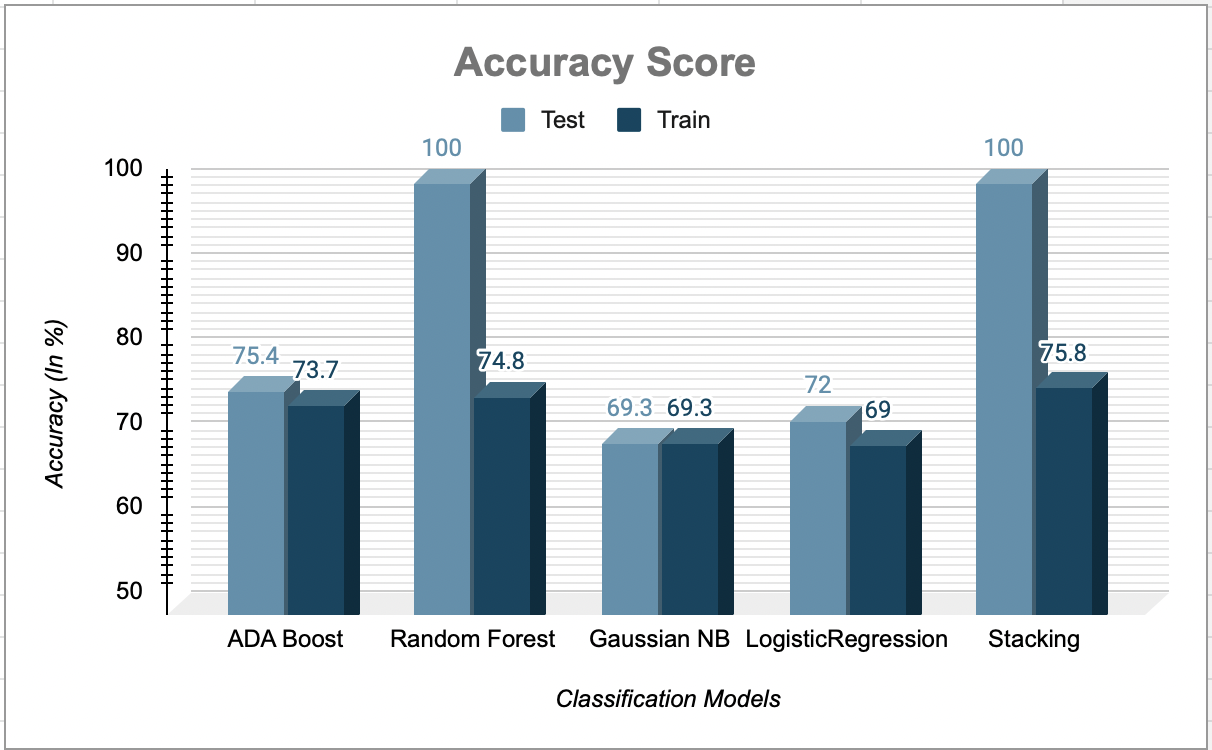
\includegraphics[width=0.7\linewidth,frame]{CA2-template/RIC15.png}
       \caption{Accuracy \label{fig:13}}
    \end{center}
\end{figure}

\subsubsection{Receiver Operating Characteristic Curve}
It is a graphical display method which, assesses the results of the binary classifier and also measures the distinct descriptors. 
The stacking classifier's ROC curve, shown in Figure \ref{fig:15}, demonstrates how well it can classify among positive as well as negative classes.
\begin{figure}[H]
    \begin{center}
        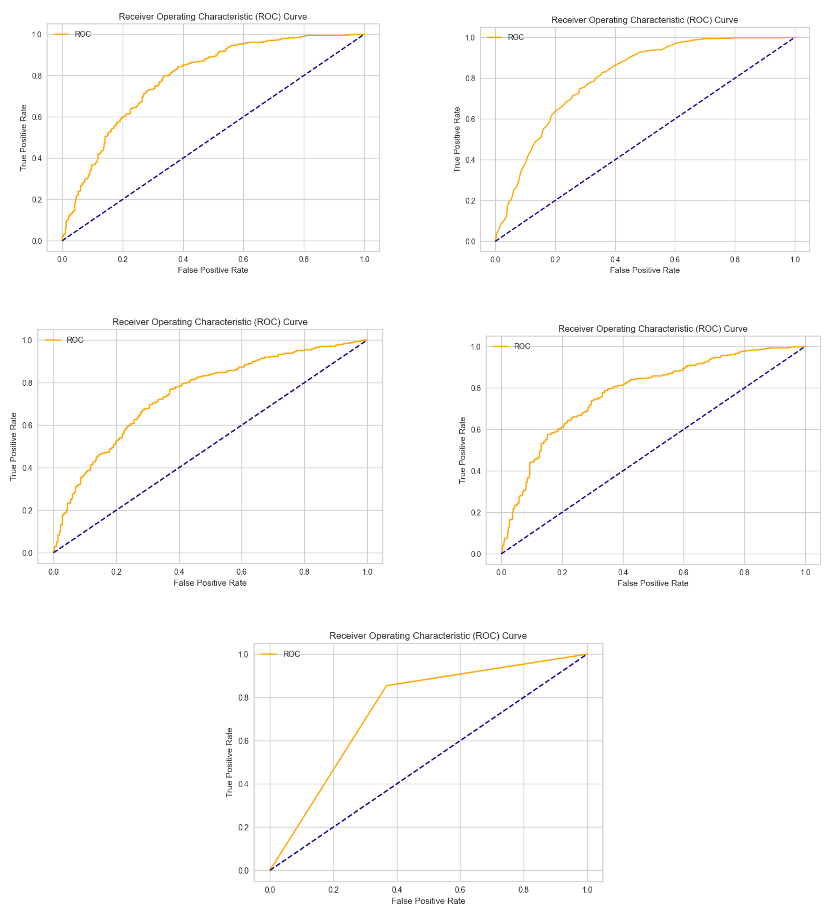
\includegraphics[width=0.7\linewidth,frame]{CA2-template/RIC17.png}
       \caption{ROC \label{fig:15}}
    \end{center}
\end{figure}

\subsubsection{Confusion Matrix}
The confusion matrix creates a connection among the labels given to a sample as well as the classifier's judgments. It is a technique for assessing the consistency of the classification scheme. Diagonally in uncertainty matrix are the cases that have been correctly classified; the other cases are incorrectly classified. 
The Figure \ref{fig:12} shows the comparison of the confusion matrices and evidently stacking classifier is performing better compared to the rest.

\begin{figure}[H]
    \begin{center}
        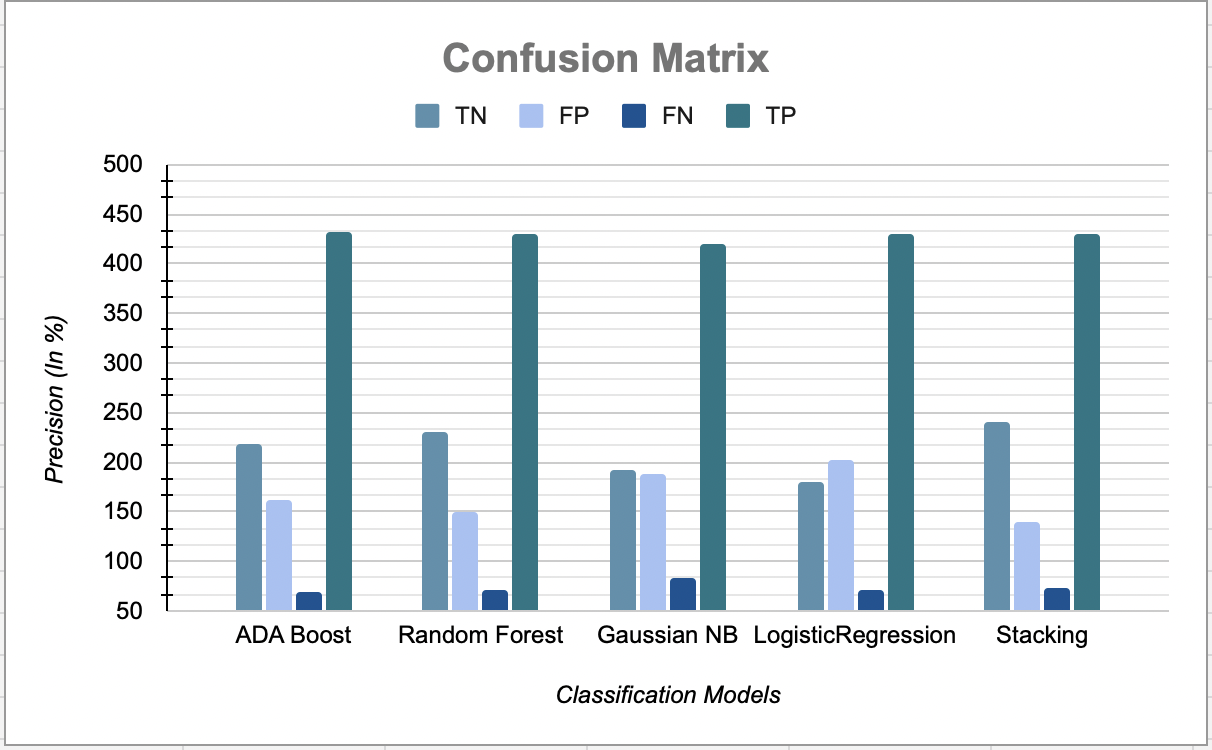
\includegraphics[width=0.7\linewidth,frame]{CA2-template/RIC13.png}
       \caption{Confusion Matrix \label{fig:12}}
    \end{center}
\end{figure}

\section{Conclusion}
As digital health-care systems are still in its infancy, experts are always cautious about processing power and latency of these systems. As a result, a system with secure fog-based telehealth as a service has been developed for real-world applications of automatic health analysis after a combined study of the major issues with the present telehealth applications. The system is given intelligence through machine learning. The SPATS framework makes use of fog computing to lower each system-related device's latency as well as bandwidth cost. By including stacking classifier, the technique for early health analysis and treatment prediction is integrated in this system. Several samples of patient's laboratory test results from a private medical center in Indonesia are included in the EHR dataset used for SPATS. Moreover , it's architecture uses AES encryption to provide users as well as their smart devices with secure and authorized access. The evaluations are conducted to test the overall efficiency of the system as well as the effectiveness of the classifier employed. The results show how the framework has been improved and show how it will successfully support smarter health care services and raise service quality.

The SPATS framework could be further improved utilizing optimization techniques because the research in this study overlooked the impact of heavy load on the system. Moreover, a totally secure telehealth system can be built by integrating homomorphic encryption for securing the personal medical data while it is in transit, at rest, and during processing.


\begin{thebibliography}{40}

\bibitem{1} X. Liang et al., “Enabling pervasive healthcare through continuous remote health monitoring,” IEEE Wireless Communications, vol. 19, no. 6, pp. 10–18, Dec. 2012, doi: 10.1109/MWC.2012.6393513.

\bibitem{0} “Entropy | Free Full-Text | Fog Computing: Enabling the Management and Orchestration of Smart City Applications in 5G Networks | HTML.” https://www.mdpi.com/1099-4300/20/1/4/htm (accessed Aug. 02, 2022).

\bibitem{3} “Fog Computing and the Internet of Things (IoT): A Review | IEEE Conference Publication | IEEE Xplore.” https://ieeexplore.ieee.org/document/9492161 (accessed Aug. 02, 2022).

\bibitem{2} T. N. Gia, M. Jiang, A.-M. Rahmani, T. Westerlund, P. Liljeberg, and H. Tenhunen, “Fog Computing in Healthcare Internet of Things: A Case Study on ECG Feature Extraction,” in 2015 IEEE International Conference on Computer and Information Technology; Ubiquitous Computing and Communications; Dependable, Autonomic and Secure Computing; Pervasive Intelligence and Computing, Oct. 2015, pp. 356–363. doi: 10.1109/CIT/IUCC/DASC/PICOM.2015.51.

\bibitem{4} S. Yi, Z. Hao, Z. Qin, and Q. Li, “Fog Computing: Platform and Applications,” in 2015 Third IEEE Workshop on Hot Topics in Web Systems and Technologies (HotWeb), Nov. 2015, pp. 73–78. doi: 10.1109/HotWeb.2015.22.

\bibitem{7} A. M.-H. Kuo, “Opportunities and Challenges of Cloud Computing to Improve Health Care Services,” J Med Internet Res, vol. 13, no. 3, p. e67, Sep. 2011, doi: 10.2196/jmir.1867.

\bibitem{10} S. H. and N. V., “A review on fog computing: Architecture, fog with iot, algorithms and research
challenges,” ICT Express, vol. 7, no. 2, pp. 162–176, 2021.

\bibitem{11} V. Dahiya and S. Dalal, “Fog computing: A review on integration of cloud computing and internet of
things,” in 2018 IEEE International Students’ Conference on Electrical, Electronics and Computer
Science (SCEECS), pp

\bibitem{12} M. Y. uddin and S. Ahmad, “A review on edge to cloud: Paradigm shift from large data centers
to small centers of data everywhere,” in 2020 International Conference on Inventive Computation
Technologies (ICICT), pp. 318–322, 2020. CORE2021= Not available, H Index: 11

\bibitem{13} M. E. IDRISSI, O. ELBEQQALI, and J. RIFFI, “From cloud computing to fog computing: two
technologies to serve iot–a review-,” in 2019 IEEE International Smart Cities Conference (ISC2),
pp. 272–279, 2019.

\bibitem{15} S. K. Sood and I. Mahajan, “Wearable iot sensor based healthcare system for identifying and
controlling chikungunya virus,” Computers in Industry, vol. 91, pp. 33–44, 2017. JCR Impact Factor
2021: 7.63

\bibitem{17} H. Ben Hassen, N. Ayari, and B. Hamdi, “A home hospitalization system based on the internet of
things, fog computing and cloud computing,” Informatics in Medicine Unlocked, vol. 20, p. 100368,
2020.JCR Impact Factor 2021: 3.8

\bibitem{18} H. Saidi, N. Labraoui, A. A. A. Ari, and D. Bouida, “Remote health monitoring system of elderly
based on fog to cloud (f2c) computing,” in 2020 International Conference on Intelligent Systems and
Computer Vision (ISCV), pp. 1–7, 2020. CORE2021= RANK C

\bibitem{22} F. Ma, J. Gao, Q. Suo, Q. You, J. Zhou, and A. Zhang, “Risk Prediction on Electronic Health Records with Prior Medical Knowledge,” in Proceedings of the 24th ACM SIGKDD International Conference on Knowledge Discovery & Data Mining, New York, NY, USA, Jul. 2018, pp. 1910–1919. doi: 10.1145/3219819.3220020.

\bibitem{23} C. K. Leung, T. H. Daniel Mai, N. D. Thong Tran, and C. Y. Zhang, “Predictive Analytics to Support Health Informatics on COVID-19 Data,” in 2021 IEEE 21st International Conference on Bioinformatics and Bioengineering (BIBE), Oct. 2021, pp. 1–9. doi: 10.1109/BIBE52308.2021.9635556.

\bibitem{25} “Getting started with Visual Studio,” Visual Studio. https://visualstudio.microsoft.com/vs/getting-started/ (accessed Aug. 03, 2022).

\bibitem{26} H. Gupta, A. Dastjerdi, S. Ghosh, and R. Buyya, “iFogSim: A Toolkit for Modeling and Simulation of Resource Management Techniques in Internet of Things, Edge and Fog Computing Environments,” Software: Practice and Experience, vol. 47, Jun. 2016, doi: 10.1002/spe.2509.

\bibitem{27} M. Sadikin, “EHR Dataset for Patient Treatment Classification,” vol. 1, May 2020, doi:
10.17632/7kv3rctx7m.1. https://data.mendeley.com/datasets/7kv3rctx7m/1

\end{thebibliography}

\end{document}